%
% Sección de estándares y recomendaciones del NIST
% Capítulo de análisis y diseño de generación de tokens.
% Proyecto Lovelace.
%

\section{Estándares y recomendaciones}
\label{sec:estandares}

\subsection{Estándares del PCI DSS}

En \cite{pci_tokens}, el \gls{gl:pci} \gls{gl:ssc} divide a los
\glspl{gl:token} en reversibles e irreversibles. A su vez, los reversibles se
dividen en criptográficos y en no criptográficos; mientras que los
irreversibles se dividen en autenticables y no autenticables (figura
\ref{fig:division_tokens}).

Los \glspl{gl:token} irreversibles no pueden, bajo ninguna circunstancia, ser
reconvertidos al \gls{gl:pan} original. Esta restricción aplica tanto para
cualquier entidad en el entorno del negocio (comerciante, proveedor de
\glspl{gl:token}, banco) como para cualquier posible atacante. Dados un
\gls{gl:pan} y un \gls{gl:token}, los identificables permiten validar cuando el
primero fue utilizado para la creación del segundo, mientras que los no
identificables, no.

% TODO: ¿Para qué demonios sirven los no identificables?
% Para absoulutamente nada... Llenar formatos sin verse descarados y poner
% puros ceros.

% TODO: este párrafo me está dando problemas. No quiero copiar tal cuál la
% clasificación del PCI sin manifestar disconformidad, pero tampoco quiero
% entrar en demasiados detalles aún sobre las propias implementaciones
% (las cuales, evidentemente, sí son criptográficas); PD: hay que citar más
% publicaciones, a parte de la de Sandra.

La clasificación del \gls{gl:pci} \gls{gl:ssc} con respecto a los reversibles
resulta un poco confusa (esto ya ha sido señalado antes, \cite{doc_sandra}).
Establece que los criptográficos son generados utilizando
\gls{gl:criptografia_fuerte}, el \gls{gl:pan} nunca se almacena, solamente se
guarda una llave; los no criptográficos guardan la relación entre
\glspl{gl:token} y \gls{gl:pan} en una base de datos. El problema está en que
no se menciona \textit{cómo} generar los no criptográficos. A pesar del nombre,
los métodos más comunes para esta categoría ocupan
\glspl{gl:primitiva_criptografica} (p. ej. generadores pseudoaleatorios); además
de que, en una implementación real, para poder cumplir con el \gls{gl:pci}
\gls{gl:dss}, la propia base de datos debe de estar cifrada \cite{pci_dss}.

\begin{figure}[h]
  \begin{center}
    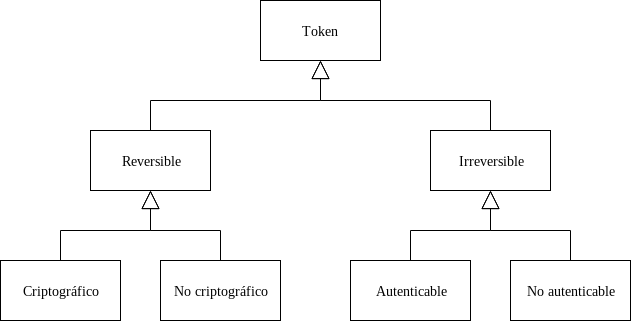
\includegraphics[width=0.75\linewidth]{diagramas/clasificacion.png}
    \caption{Clasificación de los \glspl{gl:token}
      según \gls{gl:pci} \gls{gl:ssc}.}
    \label{fig:division_tokens}
  \end{center}
\end{figure}

\subsection{Estándares del NIST}

\begin{description}

  \item[Administración de llaves] (Sección \ref{sec:administracion_llaves})
    \begin{description}
      \item[800-57] \textit{Recommendation for Key Management}. Disponible en
        \cite{nist_llaves}.
      \item[800-130] \textit{A Framework for Designing Cryptographic Key
        Management Systems}. Disponible en \cite{nist_disenio_llaves}.
    \end{description}

  \item[Generación de llaves] (Sección \ref{sec:generacion_llaves})
    \begin{description}
      \item[800-108] \textit{Recommendation for Key Derivation Functions Using
        Pseudorandom Functions}. Disponible en \cite{nist_derivacion_llaves}.
      \item[800-133] \textit{Recommendation for Cryptographic Key Generation}.
        Disponible en \cite{nist_creacion_llaves}.
    \end{description}

  \item[Generación de bits pseudoaleatorios] (Sección
    \ref{sec:generadores_pseudoaleatorios})
    \begin{description}
      \item[800-90A Revision 1] \textit{Recommendation for Random Number Generation Using
        Deterministic Random Bit Generators}. Disponible en
        \cite{nist_aleatorios}.
    \end{description}
\end{description}

\subimport{/}{administracion_llaves}
\subimport{/}{generacion_llaves}
\subimport{/}{generadores_pseudoaleatorios}
\subimport{/}{pruebas}
